\documentclass[11pt]{beamer}
\usepackage[utf8]{inputenc}
\usepackage[T1]{fontenc}
\usepackage{lmodern,graphicx}
\usetheme{Boadilla}
\begin{document}
	\author[Kumar, Bajpai]{Vineet Kumar (19BM6JP46) \\ Rohit Bajpai ~(19BM6JP56)}
	\title[Sentiment Mining of Nursing Notes]{\textbf{Sentiment Mining of Nursing Notes \\for Mortality Prediction}}
	%\subtitle{}
	%\logo{}
	%\institute{}
	\date[\today]{\colorbox{blue!10}{WorkinProgress} \normalcolor $ |$ Project for (BM60130) Healthcare Analytics}
	%\subject{}
	%\setbeamercovered{transparent}
	\setbeamertemplate{navigation symbols}{}
	\begin{frame}[plain]
		\maketitle
	\end{frame}
	
	\begin{frame}
		\frametitle{Problem Statement}
		\begin{block}~
			Using Unstructured Clinical Data (UCD) to predict mortality of patient
		\end{block}
\underline{Types of UCD:}
	Nursing Progress Note, Radiology Report etc.\pause 
	\begin{block}{Example of Nursing progress Note}
		Pt is a 57 y/p male with h/o afib, LE edema, who presented to
		cardiologist
		s office [**3-25**] c/p worsening LE edema and orthopnea. TTE
		showed R CHF and admitted
		hypoxic on admission and bradycardic in
		50s-60s. Aggressively diuresed since admission, on lasix gtt up to
		10/hour; spironolactone; diamox. He also has pulm. Hypertension.
		Triggered for somnolence  on 24th
		started on 2L of O2. On the 25th
		demonstrated diminished mental status and hypoxia in setting of CPAP,
		so it was stopped. Last night patient intolerant of mask/autoset.
		Overnight and this morning had increasing hypercarbia and marked
		somnolence to point of being obtunded. Transferred to MICU for further
		management.
		Impaired Skin Integrity
	\end{block} 
	\end{frame}
\begin{frame}{}
	\begin{block}{Using Unstructured Clinical Data to predict \textbf{mortality of patient}}
		\begin{itemize}
			\item In this work we are only considering Nursing Notes. 
			\item Mortality of Patient --- (i) 30 day mortality (ii) >30 days mortality
		\end{itemize}
	\end{block}
	
	\begin{block}{Dataset}
		\begin{itemize}
			\item We are using MIMIC - III dataset \footnote{Johnson AE, Pollard TJ, Shen L, Lehman LwH, Feng M, Ghassemi M, et al. MIMIC-III, a freely accessible critical care database. Scientific data. 2016; 3. \url{https://doi.org/10.1038/sdata.2016.35}}
			\item Access to dataset was obtained through proper channel and due compliance of ethics 
			\item Dataset contains completely anonymised data of 40,000 patients who were admitted to the
			ICUs of the Beth Israel Deaconess Medical Center between 2001 and 2012
		\end{itemize}
	\end{block}
	
	

 \end{frame}

\begin{frame}{Approach}
\begin{itemize}
	\item Uncompressed size of dataset is ~6GB
\item Data were extracted from the MIMIC database using
\textbf{Google Big Query} with the help of dialect of Structured Query Language (SQL)
\item DB contains multiple tables % TODO: \usepackage{graphicx} required
\begin{figure}
	\centering
	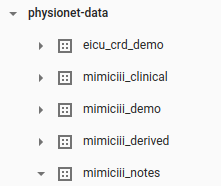
\includegraphics[width=0.2\linewidth]{db}
	\label{fig:db}
\end{figure}
using appropriate joins relevant patient notes and other information were extracted
\item Using elementry techniques polarity scores were computed
\end{itemize}

\end{frame}

\begin{frame}{Approach}
\begin{enumerate}
	\item Data Extraction from Database using Bigquery
	\item Data Preprocessing (remove stop words etc.)
	\item Sentiment Mining using LDA/Polarity and subjectivity
	\item Using RNN for lower dimensional representation and unsupervised clustering
	\item Possibly survival analysis 
\end{enumerate}
\end{frame}
\begin{frame}{Elementary Results}
	\begin{figure}
		\centering
		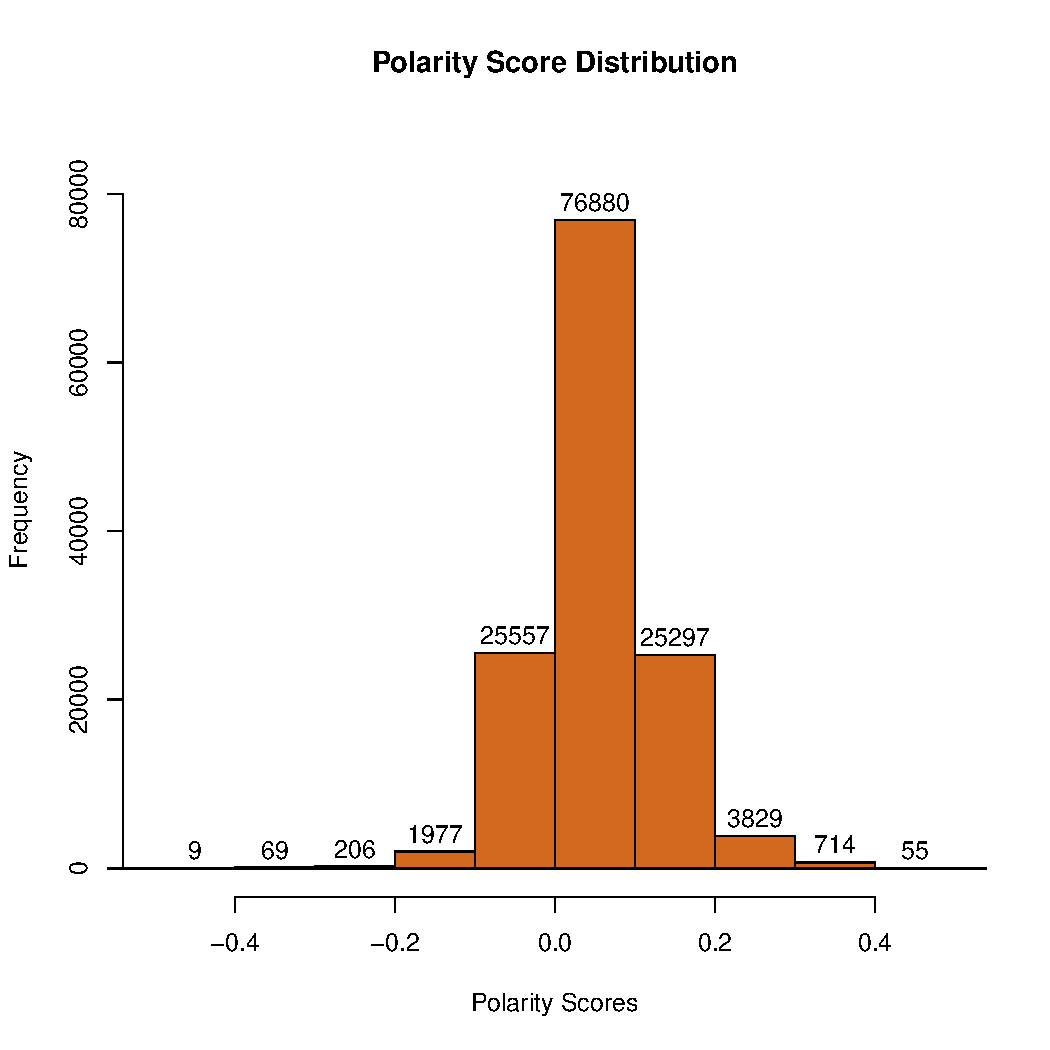
\includegraphics[width=0.48\linewidth]{pol}		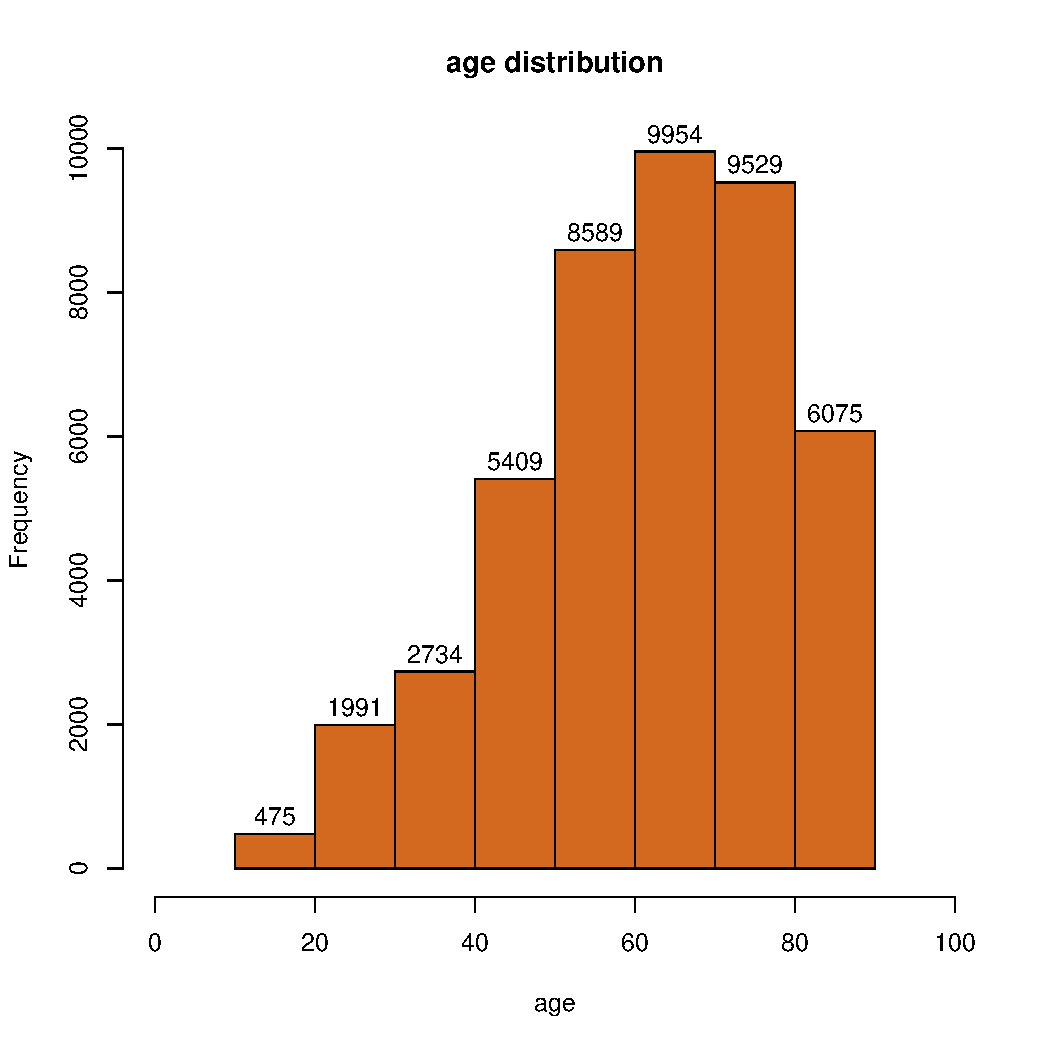
\includegraphics[width=0.48\linewidth]{../report/img/age-distr}
		\label{fig:pol}
	\end{figure}
Daily codes pushed at \url{https://github.com/vntkumar8/HealthCareAnalytics}
\end{frame}




\begin{frame}{References}
	\begin{itemize}
		\item Tran, Nam, and Joon Lee. "Using multiple sentiment dimensions of nursing notes to predict mortality in the intensive care unit." 2018 IEEE EMBS International Conference on Biomedical \& Health Informatics (BHI). IEEE, 2018.
		\item McCoy, Thomas H., et al. "Sentiment measured in hospital discharge notes is associated with readmission and mortality risk: an electronic health record study." PloS one 10.8 (2015).
		\item Ghassemi, Mohammad M., Roger G. Mark, and Shamim Nemati. "A visualization of evolving clinical sentiment using vector representations of clinical notes." 2015 Computing in cardiology conference (CinC). IEEE, 2015.
		
	\end{itemize}
\end{frame}

\end{document}